\section{Behavioral studies of retrieved guidance}
\label{sec:evidence}
\label{sec:recorded-interventions}
\label{sec:content}
The Django example in Section~\ref{sec:motivation} illustrates strategy
transfer. Here we examine how agents apply a retrieved behavioral requirement:
what context they need, which interactions they miss, and how feedback
changes the next edit. Figures~\ref{fig:concept} and~\ref{fig:behavior-workflow}
show the checks and workflow used for these studies.



\begin{figure}[!htbp]
\centering
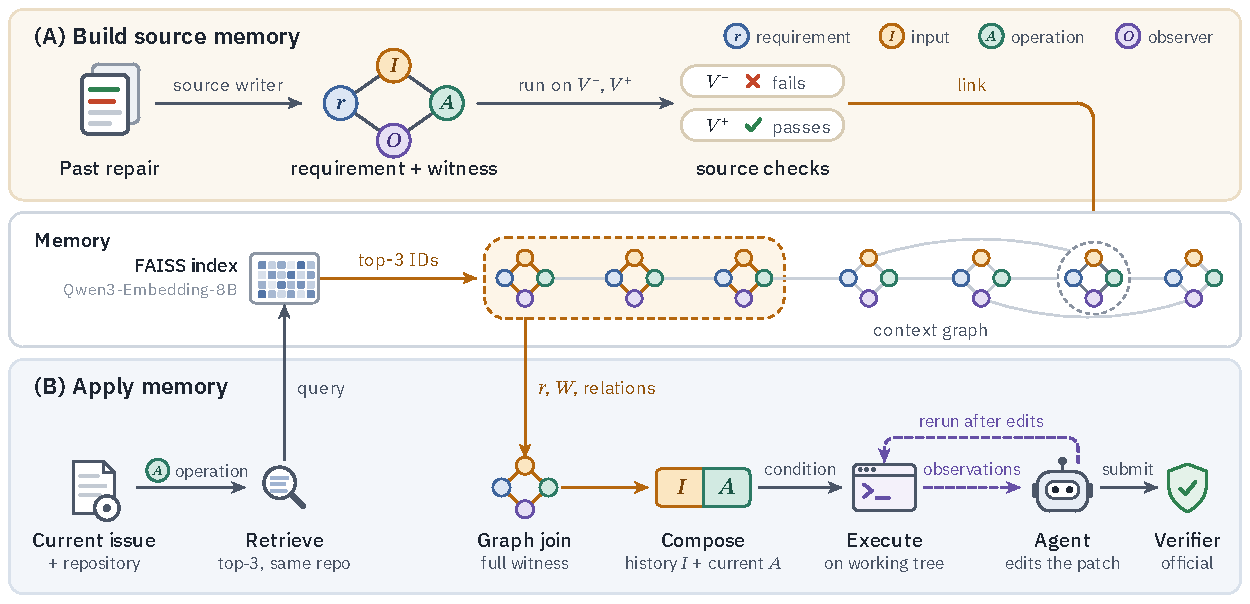
\includegraphics[width=\linewidth]{figures/contextgraph-design/fig2-overview.pdf}
\caption{Workflow for the behavioral studies. (A) Historical
repairs supply requirements and checked examples linked in memory.
(B) Retrieval selects relevant sources; graph relations support composition
with the current operation. Execution feedback guides edits before verification.}
\label{fig:behavior-workflow}
\end{figure}

\paragraph{Retain the context that makes advice useful.}
In four paired runs, memory helps preserve query strings, remove redundant
uniqueness while retaining primary keys, honor destination timezones, and
preserve named-tuple ranges (Table~\ref{tab:historicalrequirements}). Both
repairs in the first three pairs pass official verification.

\begin{table}[!htbp]
\centering
\caption{Joint current/historical behavior in complete-agent comparisons.
The columns report whether repairs with and without memory preserve both the current behavior and the historical requirement.}
\label{tab:historicalrequirements}
\begin{tabular}{llcc}
\toprule
Target & Historical addition & No memory & Memory \\
\midrule
Django14404 & Preserve query string & Fail & Pass \\
Django12708 & Delete redundant uniqueness & Fail & Pass \\
Django11138 & Honor destination timezone & Fail & Pass \\
Django12663 & Preserve named-tuple range & Fail & Pass \\
\bottomrule
\end{tabular}
\end{table}

We then vary the memory supplied for the constraint and timezone tasks:
a written requirement, implementation details, both, or neither
(Table~\ref{tab:memorycontent}). All eight repairs pass official verification.
For constraints, the requirement alone leads the agent to test different
columns and miss the same-column bug; the implementation retains that
condition. For timezones, the requirement directs the agent to a suitable
helper, whereas the old implementation leads to errors on named timezones.

\begin{table}[!htbp]
\centering
\caption{Memory-content interventions: one fresh attempt per input and development task.
All eight pass official verification. MySQL and named-zone checks were constructed
after inspecting the timezone repairs and applied to all four submissions.}
\label{tab:memorycontent}
\small
\begin{tabular}{lcccc}
\toprule
Memory input & Constraint joint & Timezone joint & MySQL cases & Named-zone cases \\
\midrule
None & Fail & Fail & Pass & Fail \\
Requirement & Fail & Pass & Pass & Pass \\
Implementation & Pass & Pass & Pass & Fail \\
Both & Pass & Pass & Fail & Pass \\
\bottomrule
\end{tabular}
\end{table}

On Django12663, both retrieved memory sets contain the relevant named-tuple
source, yet both initial repairs miss its behavior. Preserving its constructor
convention fixes named tuples while keeping ordinary subclasses working;
passing every sequence's elements as separate arguments breaks the latter
(Appendix Figure~\ref{fig:memory-content-scope}). A candidate-selection
diagnostic also shows that an exact operation filter discards this useful source
(Appendix~\ref{sec:details-evidence}).
\textbf{Finding:} advice needs its applicability context: shared columns
and constructor conventions determine how these lessons transfer.

\paragraph{Check a historical requirement in the current workflow.}
\label{sec:composition-results}
A Django12663 repair passes the current lazy-User query and historical
named-tuple example separately, but fails their combination. The range
adapter inserts the historical type into the current query, retaining the
lazy User and nested query (Figure~\ref{fig:concept}).

Three agents start from the same unrepaired code, history, current program,
tools, and instructions (Table~\ref{tab:composedconditions}). Separate
historical checks recover both historical examples but only one of three
withheld joint queries. Composed checks recover both historical examples
and all three joint queries, while preserving ordinary subclasses.

\begin{table}[!htbp]
\centering
\caption{Django12663 repairs from original code with identical history,
current program and failure, tools, and instructions. Two arms add composed
or separate historical checks. Historical examples are supplied to the corresponding arms; joint queries and ordinary subclasses are withheld. Mechanical checks probe input representations. Rows count checks, not independent tasks.}
\label{tab:composedconditions}
\begin{tabular*}{\linewidth}{@{}l@{\extracolsep{\fill}}ccc@{}}
\toprule
Measured behavior & \shortstack{Current\\feedback} & \shortstack{+ Separate\\history} & \shortstack{+ Composed\\conditions}  \\
\midrule
Official target verification & Pass & Pass & Pass \\
Supplied historical named-tuple examples & 0/2 & 2/2 & 2/2 \\
Withheld nonempty joint queries & 2/3 & 1/3 & 3/3 \\
Withheld ordinary subclasses & 2/2 & 2/2 & 2/2 \\
Mechanical scalar / named tuple / tuple & 2/3 & 2/3 & 3/3 \\
\bottomrule
\end{tabular*}
\end{table}

Timezone composition varies the database, application, and output zones.
Requirement and Both pass all 72 combinations; Implementation fails 32,
including 16 passed without memory.
\textbf{Finding:} combining a historical trigger with the current operation
exposes interactions that separate checks miss.

\paragraph{Use failure observations to guide the next edit.}
\label{sec:feedback-results}
Two fresh agents revisit the failed constraint repair with the same
requirement. Textual review fixes the primary-key case but misses the ordinary
unique-field case; adding the historical check and its failures helps the
agent distinguish constraint names and fix both. On the timezone task,
further issue-based review leaves the patch unchanged, while the historical
failure leads to a revision honoring the destination timezone.

Of four fresh refinements of the Django12663 candidate, history alone passes
all seven measured conditions in one of two attempts; the joint program and
failure do so in two of two. All four pass official verification. For the
simpler redirect task, a requirement sentence already yields the same correct
implementation as requirement-plus-feedback.
\textbf{Finding:} targeted failure feedback helps agents act on a known
requirement when textual review alone leaves the defect unresolved.
